% Includi il preambolo con tutti i pacchetti e le impostazioni
% --- Pacchetti e configurazioni di base ---
\documentclass[10pt, a4paper]{article}

% --- Lingua e codifica ---
\usepackage[utf8]{inputenc}
\usepackage[T1]{fontenc}
\usepackage[italian]{babel}

% --- Matematica e simboli ---
\usepackage{amsmath}         % Per ambienti matematici avanzati
\usepackage{amssymb}         % Per simboli matematici
\usepackage{amsfonts}        % Per i font matematici
\usepackage{xfrac}           % Per frazioni "slanted" (es. 1/2)

% --- Layout e stile ---
\usepackage[a4paper, margin=1cm]{geometry} % Margini ridotti per un cheatsheet
\usepackage{multicol}      % Per disporre il testo in più colonne
\usepackage{graphicx}      % Per includere immagini
\usepackage{parskip}       % Per avere spazio tra i paragrafi invece dell'indentazione
\usepackage{xcolor}        % Per usare i colori

% --- Intestazione e piè di pagina ---
\usepackage{fancyhdr}
\pagestyle{fancy}
\fancyhf{} % Pulisce tutte le intestazioni e i piè di pagina
\fancyhead[C]{Cheatsheet di Algoritmi e Strutture Dati}
\fancyfoot[C]{\thepage}
\renewcommand{\headrulewidth}{0.4pt}
\renewcommand{\footrulewidth}{0.4pt}

% --- Link e riferimenti ---
\usepackage{hyperref}
\hypersetup{
    colorlinks=true,
    linkcolor=blue,
    filecolor=magenta,
    urlcolor=cyan,
}

% --- Comandi personalizzati (utili per la matematica) ---
\newcommand{\bigO}[1]{\mathcal{O}(#1)}
\newcommand{\bigOmega}[1]{\Omega(#1)}
\newcommand{\bigTheta}[1]{\Theta(#1)}

% Inizio del documento
\begin{document}

% --- Pagina del titolo ---
\begin{titlepage}
    \maketitle
    \thispagestyle{empty}  % <-- Questo comando rimuove il piè di pagina dalla pagina del titolo
\end{titlepage}

% --- Sezione Complessità ---
\section{Complessità}
\subsection{Notazioni di Complessità Asintotica in Elenco}

\begin{itemize}
    \item $f(n) = O(g(n))$ - \textbf{O grande} - Limite asintotico superiore
    \item $f(n) = \Omega(g(n))$ - \textbf{Omega grande} - Limite asintotico inferiore
    \item $f(n) = \Theta(g(n))$ - \textbf{Theta grande} - Limite asintotico sia superiore che inferiore
\end{itemize}

\subsection{Confronto Tramite Limiti}
Dato il limite $L = \lim_{n\to\infty} \frac{f(n)}{g(n)}$:
\begin{itemize}
    \item Se $L = 0$, allora $\Theta(f(n)) < \Theta(g(n))$.
    \item Se $L = c$ (con $c \neq 0, \infty$), allora $\Theta(f(n)) = \Theta(g(n))$.
    \item Se $L = \infty$, allora $\Theta(f(n)) > \Theta(g(n))$.
\end{itemize}

\subsection{Gerarchia Fondamentale degli Ordini di Grandezza}
Per costanti $k,h \in \mathbb{R}^+$ e $a>1$:
$$ \Theta(1) < \Theta((\log n)^{k}) < \Theta(n^{h}) < \Theta(a^{n}) < \Theta(n!) < \Theta(n^{n}) $$

\subsection{Complessità degli Automi}
\begin{itemize}
    \item \textbf{DFSA (Automa a Stati Finiti Deterministico)}
    \begin{itemize}
        \item Complessità Temporale: $T_A(n) = \Theta(n)$
        \item Complessità Spaziale: $S_A(n) = \Theta(1)$
    \end{itemize}

    \item \textbf{DPDA (Automa a Pila Deterministico)}
    \begin{itemize}
        \item Complessità Temporale: $T_A(n) = \Theta(n)$
        \item Complessità Spaziale: $\Theta(0) \le \Theta(S_A(n)) \le \Theta(n)$
    \end{itemize}

    \item \textbf{k-DTM (Macchina di Turing Deterministica a k-nastri)}
    \begin{itemize}
        \item Complessità Temporale: Nessun limite generale.
        \item Complessità Spaziale: $\Theta(S_M(n)) \le \Theta(T_M(n))$
    \end{itemize}

    \item \textbf{SDTM (Macchina di Turing Deterministica a nastro singolo)}
    \begin{itemize}
        \item Complessità Temporale: Nessun limite generale.
        \item Complessità Spaziale: $S_M(n) = \Omega(n)$
    \end{itemize}
\end{itemize}

\subsection{Complessità delle RAM}

\subsubsection{Criteri di Costo}
\begin{itemize}
    \item \textbf{Costo Costante:} Ogni istruzione ha costo 1. Ogni cella di memoria ha costo 1, indipendentemente dal valore contenuto.
    \item \textbf{Costo Logaritmico:} Il costo di un'operazione e dello spazio occupato dipende dalla dimensione (logaritmo) dei valori numerici coinvolti.
    $$
    l(x) := 
    \begin{cases}
        \lfloor \log_2 x \rfloor + 1 & \text{se } x \neq 0 \\
        1 & \text{se } x = 0
    \end{cases}
    \quad \text{N.B.: } l(x) = \Theta(\log x)
    $$
    \item \textbf{Quando sceglierli:} I due criteri sono equivalenti se la dimensione degli operandi è limitata da una costante. Se i numeri possono diventare arbitrariamente grandi, il criterio logaritmico è più realistico.
\end{itemize}

\subsubsection{Calcolo del Costo Logaritmico (caso semplificato)}
Sotto l'ipotesi di usare un numero costante di celle di memoria:
\begin{itemize}
    \item \textbf{Costo Spaziale:} Lo spazio totale è la somma della "lunghezza" (logaritmo) di tutti i numeri più grandi salvati in ogni cella di memoria utilizzata.
    \item \textbf{Gestione di un intero i} (es. \texttt{LOAD, STORE, READ, WRITE, JZ})
    \begin{itemize}
        \item Costo Temporale: $\Theta(\log i)$
    \end{itemize}
    \item \textbf{Operazioni Aritmetiche} (su operandi $n_1, n_2$)
    \begin{itemize}
        \item Addizione (+), Sottrazione (-): $\Theta(\log n_1 + \log n_2)$
        \item Moltiplicazione (*), Divisione (/): $\Theta(\log n_1 \cdot \log n_2)$
    \end{itemize}
\end{itemize}

\subsection{Classi di Complessità Comuni}
\begin{itemize}
    \item $\mathcal{O}(1)$: Costante (es. accesso a un elemento di un array)
    \item $\mathcal{O}(\log n)$: Logaritmica (es. ricerca binaria)
    \item $\mathcal{O}(n)$: Lineare (es. scansione di una lista)
    \item $\mathcal{O}(n \log n)$: Lineare-logaritmica (es. merge sort, heapsort)
    \item $\mathcal{O}(n^2)$: Quadratica (es. bubble sort, selection sort)
    \item $\mathcal{O}(2^n)$: Esponenziale (es. problemi risolti con la forza bruta)
    \item $\mathcal{O}(n!)$: Fattoriale (es. problema del commesso viaggiatore con forza bruta)
\end{itemize}
\newpage

% --- Sezione Complessità ---
\section{TM}
\subsection{Complessità degli Automi}
\begin{itemize}
    \item \textbf{DFSA (Automa a Stati Finiti Deterministico)}
    \begin{itemize}
        \item Complessità Temporale: $T_A(n) = \Theta(n)$
        \item Complessità Spaziale: $S_A(n) = \Theta(1)$
    \end{itemize}

    \item \textbf{DPDA (Automa a Pila Deterministico)}
    \begin{itemize}
        \item Complessità Temporale: $T_A(n) = \Theta(n)$
        \item Complessità Spaziale: $\Theta(0) \le \Theta(S_A(n)) \le \Theta(n)$
    \end{itemize}

    \item \textbf{k-DTM (Macchina di Turing Deterministica a k-nastri)}
    \begin{itemize}
        \item Complessità Temporale: Nessun limite generale. Per calcolarla devi immaginare il funzionamento della macchina.
        \item Complessità Spaziale: $\Theta(S_M(n)) \le \Theta(T_M(n))$
    \end{itemize}

    \item \textbf{SDTM (Macchina di Turing Deterministica a nastro singolo)}
    \begin{itemize}
        \item Complessità Temporale: Nessun limite generale. Per calcolarla devi immaginare il funzionamento della macchina.
        \item Complessità Spaziale: $S_M(n) = \Omega(n)$, ciò significa che la complessità spaziale dev'essere almeno lineare, questo perché il nastro di input coincide con il nastro di memoria.
    \end{itemize}
\end{itemize}

\textbf{TIP}: per il calcolo della complessità spaziale, ricordati di considerare il caso peggiore. Il caso peggiore può anche essere per una stringa che non viene accettata, ovvero $x \notin L$.
\newpage

% --- Sezione Complessità ---
\section{RAM}
\subsection{Complessità delle RAM}

\subsubsection{Criteri di Costo}
\begin{itemize}
    \item \textbf{Costo Costante:} Ogni istruzione ha costo 1. Ogni cella di memoria ha costo 1, indipendentemente dal valore contenuto.
    \item \textbf{Costo Logaritmico:} Il costo di un'operazione e dello spazio occupato dipende dalla dimensione (logaritmo) dei valori numerici coinvolti.
    $$
    l(x) := 
    \begin{cases}
        \lfloor \log_2 x \rfloor + 1 & \text{se } x \neq 0 \\
        1 & \text{se } x = 0
    \end{cases}
    \quad \text{N.B.: } l(x) = \Theta(\log x)
    $$
    \item \textbf{Quando sceglierli:} I due criteri sono equivalenti se la dimensione degli operandi è limitata da una costante. Se i numeri possono diventare arbitrariamente grandi, il criterio logaritmico è più realistico.
\end{itemize}

\subsubsection{Calcolo del Costo Logaritmico (caso semplificato)}
Sotto l'ipotesi di usare un numero costante di celle di memoria:
\begin{itemize}
    \item \textbf{Costo Spaziale:} Lo spazio totale è la somma della "lunghezza" (logaritmo) di tutti i numeri più grandi salvati in ogni cella di memoria utilizzata.
    \item \textbf{Gestione di un intero i} (es. \texttt{LOAD, STORE, READ, WRITE, JZ})
    \begin{itemize}
        \item Costo Temporale: $\Theta(\log i)$
    \end{itemize}
    \item \textbf{Operazioni Aritmetiche} (su operandi $n_1, n_2$)
    \begin{itemize}
        \item Addizione (+), Sottrazione (-): $\Theta(\log n_1 + \log n_2)$
        \item Moltiplicazione (*), Divisione (/): $\Theta(\log n_1 \cdot \log n_2)$
    \end{itemize}
\end{itemize}


\newpage

% --- Sezione Equazioni di Ricorrenza ---
\section{Equazioni di Ricorrenza}
\subsection{Algoritmo Divide et Impera}
Un algoritmo che segue la strategia \textit{divide et impera} si articola in tre fasi:
\begin{itemize}
    \item \textbf{Dividi:} Il problema è scomposto in sottoproblemi più semplici della stessa forma.
    \item \textbf{Impera:} I sottoproblemi vengono risolti ricorsivamente.
    \item \textbf{Combina:} Le soluzioni dei sottoproblemi sono combinate per ottenere la soluzione del problema originale.
\end{itemize}
La sua complessità temporale $T(n)$ è descritta da un'equazione di ricorrenza, tipicamente nella forma $T(n) = a \cdot T(n/b) + f(n)$.

\subsection{Metodi di Risoluzione delle Ricorrenze}

\subsubsection{Risoluzione Diretta Esplicita}
Consiste nello sviluppare iterativamente la ricorrenza fino a individuare un modello generale per esprimerne l'ordine di grandezza.

\subsubsection{Metodo di Sostituzione}
Consiste nel formulare un'ipotesi per la soluzione e nel verificarla rigorosamente tramite dimostrazione per induzione.

\subsubsection{Metodo dell'Albero di Ricorsione}
È una tecnica visuale per sviluppare le chiamate ricorsive e sommarne i costi livello per livello. È utile per formulare un'ipotesi di soluzione, da verificare poi con il metodo di sostituzione. Esempio di albero:
\begin{figure}[h!]
    \centering
    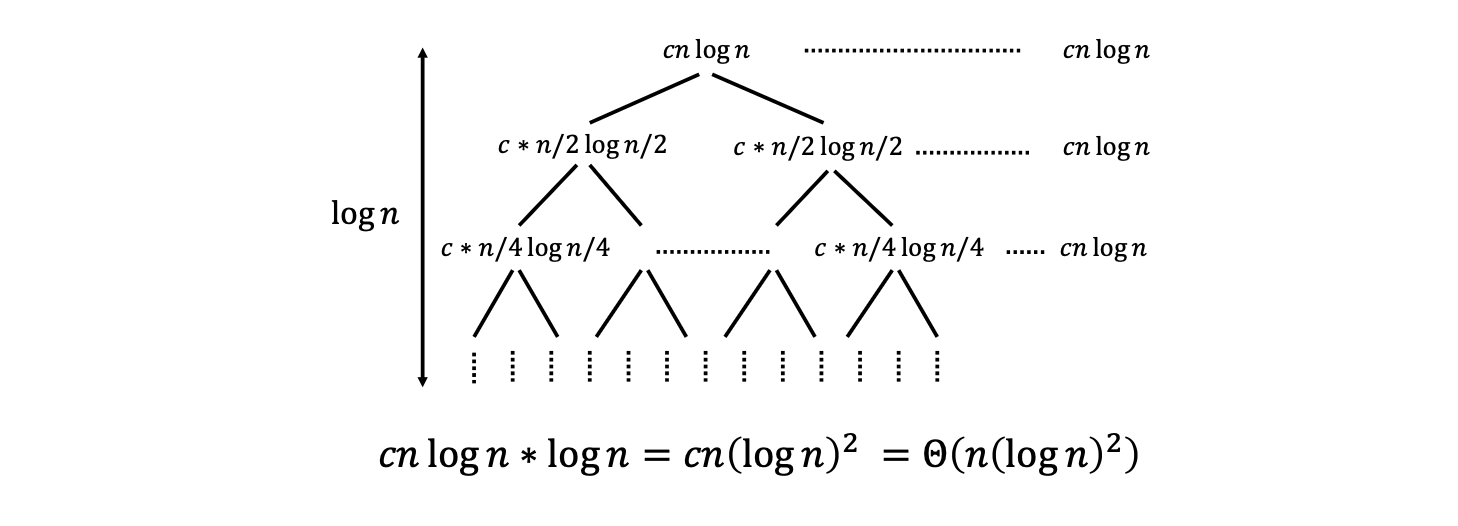
\includegraphics[width=0.8\textwidth]{images/albero_delle_ricorrenze.png}
    \caption{Esempio di un albero di ricorsione.}
    \label{fig:albero_ricorrenze}
\end{figure}

\subsubsection{Metodo per Ricorrenze Lineari}
Si applica a ricorrenze della forma $T(n) = \sum_{i=1}^{h} a_i T(n-i) + cn^k$. Posto $a := \sum a_i$, la soluzione (come limite superiore) è:
\begin{itemize}
    \item $T(n) = O(n^{k+1})$ se $a=1$.
    \item $T(n) = O(n^k a^n)$ se $a \ge 2$.
\end{itemize}

\subsubsection{Teorema Master}
Fornisce una soluzione "pronta" per ricorrenze della forma $T(n) = a \cdot T(n/b) + f(n)$ (con $a \ge 1, b > 1$). Si confronta $f(n)$ con $n^{\log_b a}$:
\begin{itemize}
    \item \textbf{Caso 1:} Se $f(n) = O(n^{\log_b a - \epsilon})$ per qualche $\epsilon > 0$, allora $T(n) = \Theta(n^{\log_b a})$.
    \item \textbf{Caso 2:} Se $f(n) = \Theta(n^{\log_b a})$, allora $T(n) = \Theta(n^{\log_b a} \log n)$.
    \item \textbf{Caso 3:} Se $f(n) = \Omega(n^{\log_b a + \epsilon})$ per qualche $\epsilon > 0$ e se $f(n)$ soddisfa una condizione di regolarità, allora $T(n) = \Theta(f(n))$.
\end{itemize}
\newpage

% --- Sezione Pseudocodice ---
\section{Pseudocodice}
\subsection{Sintassi di base}

\begin{multicols}{2} % Inizio ambiente a due colonne

\begin{itemize}
    \item \textbf{Riga di commento}
    \begin{lstlisting}
//...
    \end{lstlisting}
    \item \textbf{Assegnamento}
    \begin{lstlisting}
i := j
    \end{lstlisting}
    \item \textbf{Operazioni}
    \begin{lstlisting}
+, -, *, /, %
    \end{lstlisting}
    \item \textbf{Confronto di interi}
    \begin{lstlisting}
>, <, >=, <=, =, !=
    \end{lstlisting}
    \item \textbf{Lettura dell'input}
    \begin{lstlisting}
x := read()
    \end{lstlisting}
    \item \textbf{Restituzione in output}
    \begin{lstlisting}
return x
    \end{lstlisting}
\end{itemize}

\end{multicols}

\subsection{Istruzioni comuni}

\begin{multicols}{2} % Inizio ambiente a due colonne

\begin{itemize}
    \item \textbf{If-else}
    \begin{lstlisting}
if condizione
    istruzioni
else
    istruzioni
    \end{lstlisting}
    \item \textbf{Cicli}
    \begin{lstlisting}
while condizione
    istruzioni

for i := n_1 to n_2
    istruzioni
    \end{lstlisting}
\end{itemize}

\end{multicols}

\subsection{Oggetti e variabili}

\begin{multicols}{2} % Inizio ambiente a due colonne

\begin{itemize}
    \item I dati composti sono organizzati come oggetti. Gli oggetti hanno attributi (campi):
    \begin{itemize}
        \item \texttt{x.attr} è il valore dell'attributo \texttt{attr} dell'oggetto \texttt{x}.
    \end{itemize}
    \item Gli array sono oggetti, dotati dell'attributo \texttt{length}.
    \begin{itemize}
        \item \(A[j]\) è l'elemento di indice \(j\) dell'array A.
        \item \(A[i..j]\) è il sottoarray di A dall'i-esimo al j-esimo elemento.
    \end{itemize}
    \item Una variabile che corrisponde ad un oggetto è un puntatore all'oggetto.
    \begin{itemize}
        \item Dopo le istruzioni \( y := x, x.attr := 3 \) si ha \( y.attr = x.attr = 3 \).
    \end{itemize}
    \item Un puntatore che non fa riferimento ad alcun oggetto ha valore NIL.
    \item Usa l'istruzione \texttt{$ALLOCATE(varname, length)$} per creare un nuovo array.
\end{itemize}

\end{multicols}

\newpage

% --- Sezione Algoritmi di Ordinamento
\section{Algoritmi di Ordinamento}
\subsection{Algoritmi comuni}

\begin{center}
    \begin{tabular}{|l|c|c|}
        \hline
        \textbf{Algoritmo} & \textbf{Complessità temporale} & \textbf{Complessità spaziale} \\
        \hline
        Insertion sort & $\Theta(n^2)$ & $\Theta(1)$ \\
        \hline
        Merge sort & $\Theta(n \log n)$ & $\Theta(n)$ \\
        \hline
        Heapsort & $\Theta(n \log n)$ & $\Theta(1)$ \\
        \hline
        Quicksort & $\Theta(n^2)$ & $\Theta(1)$ \\
        \hline
        Counting sort & $\Theta(n+k)$ & $\Theta(k)$ \\
        \hline
    \end{tabular}
\end{center}

% TODO add LIN-SEARCH
% TODO inserisci qui altri algoritmi come il BIN-SEARCH che posso usare negli algoritmi per fare cose.

\subsection{Come Riconoscere la Complessità Logaritmica}

Un algoritmo ha complessità logaritmica quando il problema si riduce in modo esponenziale a ogni passo. I principali indizi nel codice sono:

\begin{itemize}
    \item \textbf{La variabile del ciclo moltiplica o divide.}
        \begin{itemize}
            \item L'aggiornamento non è un'addizione/sottrazione (es. \texttt{i := i + 1}).
            \item L'aggiornamento è una moltiplicazione o divisione per una costante $c > 1$ (es. \texttt{i := i * 2} oppure \texttt{i := i / 2}).
            \item La variabile "salta" verso il valore finale, invece di "camminare". Questo richiede $\Theta(\log n)$ passi.
        \end{itemize}
    
    \item \textbf{Lo spazio del problema viene ridotto di una frazione costante.}
        \begin{itemize}
            \item L'algoritmo scarta una porzione significativa dei dati a ogni iterazione (es. metà, un terzo, etc.).
            \item L'esempio classico è la Ricerca Binaria, che dimezza lo spazio di ricerca a ogni passo.
            \item La ricorrenza associata è spesso nella forma $T(n) = T(n/b) + O(1)$, la cui soluzione è $\Theta(\log n)$.
        \end{itemize}

    \item \textbf{Caso speciale ($\log \log n$): la variabile esegue un "super-salto".}
        \begin{itemize}
            \item La variabile di controllo viene elevata a una potenza, tipicamente al quadrato (es. \texttt{i := i * i}).
            \item La crescita è doppiamente esponenziale, portando a una complessità ancora minore di $\Theta(\log \log n)$.
        \end{itemize}
\end{itemize}

\newpage

% --- Sezione Strutture Dati ---
\section{Strutture Dati}
\subsection{Vettori (Array)}
\begin{itemize}
    \item \texttt{A.length} = lunghezza dell'array.
    \item \texttt{A[i]} = accesso a elemento \texttt{i} dell'array.
    \item \texttt{A[i..j]} = sottoarray da \texttt{i} a \texttt{j}.
    \item \texttt{n} = dimensione dell'array che è uguale a \texttt{A.length}.
\end{itemize}

\subsection{Matrici}
\begin{itemize}
    \item \texttt{M.height} = numero di righe.
    \item \texttt{M.width} = numero di colonne.
    \item \texttt{M[i][j]} = accesso a riga i colonna j.
    \item \texttt{n} = dimensione dell'input che è uguale al numero di elementi, ovvero $M.\texttt{height} \times M.\texttt{width}$.
    \item $n := M.\texttt{size}$ per una matrice quadrata, dove \texttt{size} è il numero di righe (o colonne).
\end{itemize}

\subsection{Liste Concatenate}
\begin{itemize}
    \item \texttt{L.head} = puntatore alla testa della lista.
    \item \texttt{x\_f.next = NIL}, dove \texttt{x\_f} è l'ultimo elemento della lista.
\end{itemize}

\subsubsection{Liste Singolarmente Concatenate}
\begin{itemize}
    \item \texttt{x.key} = dato contenuto nell'elemento $x$.
    \item \texttt{x.next} = puntatore all'elemento successivo.
\end{itemize}

\subsubsection{Liste Doppiamente Concatenate}
\begin{itemize}
    \item \texttt{x.key} = dato contenuto nell'elemento $x$.
    \item \texttt{x.next} = puntatore all'elemento successivo.
    \item \texttt{x.prev} = puntatore all'elemento precedente.
    \item \texttt{L.head.prev = NIL}.
\end{itemize}

\subsubsection{Liste Doppiamente Concatenate Circolari}
\begin{itemize}
    \item Utilizzano un nodo speciale detto \textbf{sentinella} (\texttt{L.nil}) al posto di \texttt{L.head}.
    \item \texttt{L.nil.key = NIL}.
    \item \texttt{L.nil.next} punta alla testa della lista.
    \item \texttt{L.nil.prev} punta alla coda della lista.
    \item La lista è "circolare": la \texttt{prev} della testa e la \texttt{next} della coda puntano a \texttt{L.nil}.
    \item Se la lista è vuota, \texttt{L.nil} punta a se stesso.
\end{itemize}

\subsection{Tabelle Hash}
\begin{itemize}
    \item \texttt{T} = array di \texttt{m} celle (slot) che memorizza i dati.
    \item \texttt{h(k)} = funzione hash che mappa una chiave \texttt{k} a un indice della tabella.
    \item \texttt{$\alpha=n/m$} = fattore di carico, definito come rapporto tra elementi e slot.
\end{itemize}

% TODO inserisci qui l'indirizzamento aperto con ispezione lineare, indirizzamento aperto con double hashing, concatenamento, indirizzamento aperto con ispezione quadratica.

\subsection{Alberi}

\subsubsection{Alberi Binari di Ricerca (BST)}
\begin{itemize}
    \item \texttt{T.root} = puntatore alla radice dell'albero.
    \item \texttt{x.key} = chiave del nodo \texttt{x}.
    \item \texttt{x.p} = puntatore al nodo padre.
    \item \texttt{x.left} = puntatore al figlio sinistro.
    \item \texttt{x.right} = puntatore al figlio destro.
    \item \texttt{x.leftsize} = (opzionale) dimensione del sottoalbero sinistro del nodo.
\end{itemize}

% TODO aggiungi gli Algoritmi di attraversamento
% TODO aggiungi i Dynamic set operations

\subsubsection{Alberi di Ricerca Generici (GST)}
\begin{itemize}
    \item \texttt{T.root} = puntatore alla radice dell'albero.
    \item \texttt{x.key} = chiave del nodo \texttt{x}.
    \item \texttt{x.p} = puntatore al nodo padre.
    \item \texttt{x.fs} = puntatore al figlio più a sinistra (first son).
    \item \texttt{x.lb} = puntatore al fratello a sinistra (left brother).
    \item \texttt{x.rb} = puntatore al fratello a destra (right brother).
\end{itemize}

\subsubsection{Alberi Rosso-Neri (RBT)}
\begin{itemize}
    \item Un RBT è un BST con attributi e proprietà aggiuntive.
    \item \texttt{T.nil} = nodo speciale \textbf{sentinella} che sostituisce i puntatori a \texttt{NIL}. Il suo colore è sempre \texttt{BLACK}.
    \item \texttt{x.color} = attributo di ogni nodo che può essere \texttt{RED} o \texttt{BLACK}.
    \item \texttt{bh(x)} = \textbf{altezza nera} del nodo, ovvero il numero di nodi neri in ogni cammino da \texttt{x} (escluso) a \texttt{T.nil} (incluso).
\end{itemize}

\paragraph{Proprietà RB}
\begin{itemize}
    \item Ogni nodo è \textbf{rosso o nero}.
    \item La \textbf{radice è nera} (\texttt{T.root.color = BLACK}).
    \item Ogni foglia (il nodo sentinella \texttt{T.nil}) è \textbf{nera}.
    \item Se un nodo è rosso, allora entrambi i suoi \textbf{figli sono neri}.
    \item Per ogni nodo, tutti i cammini semplici da quel nodo alle foglie discendenti contengono lo \textbf{stesso numero di nodi neri}.
\end{itemize}

\subsection{Grafi}

% TODO inserire le cose importanti qui.
\newpage

% --- Sezione Progetta Strutture Dati ---
\section{Progetta Strutture Dati}
\subsubsection{Complessità Vettori (Array)}

\begin{tabular}{|l|c|c|}
\hline
 & \shortstack{Non Ordinato} & \shortstack{Ordinato} \\
\hline
SEARCH (A, x) & $\Theta(n)$ & $\Theta(\log n)$ \\
\hline
INSERT (A, x) & $\Theta(1)^{*}$ & $\Theta(n)$ \\
\hline
DELETE (A, x) & $\Theta(n)$ & $\Theta(n)$ \\
\hline
SUCCESSOR (A, x) & $\Theta(n)$ & $\Theta(1)$ \\
\hline
PREDECESSOR (A, x) & $\Theta(n)$ & $\Theta(1)$ \\
\hline
MINIMUM (A) & $\Theta(n)$ & $\Theta(1)$ \\
\hline
MAXIMUM (A) & $\Theta(n)$ & $\Theta(1)$ \\
\hline
\end{tabular}

\vspace{2mm}
\footnotesize{* L'inserimento in un vettore non ordinato ha complessità $\Theta(1)$ solo se avviene in coda (append). Se l'inserimento avviene in una posizione specifica, la complessità è $\Theta(n)$ a causa della necessità di spostare gli elementi successivi.}

\subsubsection{Complessità Matrici}

\begin{tabular}{|l|c|c|}
\hline
 & \shortstack{Non Ordinata} & \shortstack{Ordinata$^{**}$} \\
\hline
SEARCH (M, x) & $\Theta(n \cdot m)$ & $\Theta(n+m)$ \\
\hline
ACCESS (M, i, j) & $\Theta(1)$ & $\Theta(1)$ \\
\hline
\end{tabular}

\vspace{2mm}
\footnotesize{** Per matrice ordinata si intende una matrice $n \times m$ in cui gli elementi sono in ordine crescente lungo ogni riga e lungo ogni colonna. L'algoritmo di ricerca con complessità $\Theta(n+m)$ parte da un angolo (es. in alto a destra) e ad ogni passo elimina una riga o una colonna. Questo approccio è valido anche per matrici con ordinamento misto (crescente sulle righe, decrescente sulle colonne).}

\subsubsection{Complessità Liste Concatenate}

\begin{tabular}{|l|c|c|c|c|}
\hline
 & \shortstack{Unsorted, \\ Singly linked} & \shortstack{Sorted, \\ Singly linked} & \shortstack{Unsorted, \\ Doubly linked} & \shortstack{Sorted, \\ Doubly linked} \\
\hline
SEARCH (L,k) & $\Theta(n)$ & $\Theta(n)$ & $\Theta(n)$ & $\Theta(n)$ \\
\hline
INSERT (L,x) & $\Theta(1)$ & $\Theta(n)$ & $\Theta(1)$ & $\Theta(n)$ \\
\hline
DELETE (L,x) & $\Theta(n)$ & $\Theta(n)$ & $\Theta(1)$ & $\Theta(1)$ \\
\hline
SUCCESSOR (L,x) & $\Theta(n)$ & $\Theta(1)$ & $\Theta(n)$ & $\Theta(1)$ \\
\hline
PREDECESSOR (L,x) & $\Theta(n)$ & $\Theta(n)$ & $\Theta(n)$ & $\Theta(1)$ \\
\hline
MAXIMUM (L) & $\Theta(n)$ & $\Theta(n)$ & $\Theta(n)$ & $\Theta(n)$ \\
\hline
MINIMUM (L) & $\Theta(n)$ & $\Theta(1)$ & $\Theta(n)$ & $\Theta(1)$ \\
\hline
\end{tabular}

\subsubsection{Complessità Tabelle Hash}

\begin{tabular}{|l|c|}
\hline
\textbf{Operazione} & \textbf{Complessità (caso medio)} \\
\hline
SEARCH (T, k) & $\Theta(1+\alpha)$ \\
\hline
INSERT (T, x) & $\Theta(1+\alpha)$ \\
\hline
DELETE (T, x) & $\Theta(1+\alpha)$ \\
\hline
\end{tabular}

\vspace{2mm}
\footnotesize{La complessità media delle operazioni in una tabella hash dipende dal fattore di carico $\alpha = n/m$ (elementi/slot). I valori indicati si riferiscono a una tabella con risoluzione delle collisioni tramite concatenamento. Per l'inserimento e la cancellazione in liste non ordinate, la complessità può essere $\Theta(1)$. Nel caso peggiore, tutte le operazioni possono degradare a $\Theta(n)$.}

\subsubsection{Complessità Alberi Binari di Ricerca (BST)}

\begin{tabular}{|l|c|}
\hline
\textbf{Operazione} & \textbf{Complessità} \\
\hline
SEARCH (T, k) & $\Theta(h)$ \\
\hline
INSERT (T, z) & $\Theta(h)$ \\
\hline
DELETE (T, z) & $\Theta(h)$ \\
\hline
MINIMUM (T) & $\Theta(h)$ \\
\hline
MAXIMUM (T) & $\Theta(h)$ \\
\hline
SUCCESSOR (T, x) & $\Theta(h)$ \\
\hline
PREDECESSOR (T, x) & $\Theta(h)$ \\
\hline
\end{tabular}

\vspace{2mm}
\footnotesize{La complessità delle operazioni su un Albero Binario di Ricerca (BST) dipende dall'altezza $h$ dell'albero. Nel caso peggiore (albero sbilanciato, simile a una catena lineare), $h = \Theta(n)$. Se l'albero è bilanciato, $h = \Theta(\log n)$.}


\end{document}